\documentclass[11pt, letterpaper]{article}

\usepackage{arxiv}
\usepackage{algorithm}
\usepackage{algorithmicx}
\usepackage{algpseudocode}
\usepackage[utf8]{inputenc} % allow utf-8 input
\usepackage[T1]{fontenc}    % use 8-bit T1 fonts
\usepackage{hyperref}       % hyperlinks
\usepackage{url}            % simple URL typesetting
\usepackage{booktabs}       % professional-quality tables
\usepackage{amsfonts}       % blackboard math symbols
\usepackage{nicefrac}       % compact symbols for 1/2, etc.
\usepackage{microtype}      % microtypography
\usepackage{multirow}
\usepackage{lipsum}		% Can be removed after putting your text content
\usepackage{graphicx}
\usepackage{natbib}
\usepackage{doi}

\title{Reinforcement Learning for Freeway Variable Speed Limit Control: A Mixed Traffic Flow Case Study}

%\date{September 9, 1985}	% Here you can change the date presented in the paper title
%\date{} 					% Or removing it

\author{ \href{https://orcid.org/0000-0003-0831-1244}{\includegraphics[scale=0.06]{orcid.pdf}\hspace{1mm}Juanwu Lu} \\
	Department of Civil and Environmental Engineering\\
	University of California, Berkeley\\
	Berkeley, CA 94720, United States \\
	\texttt{juanwu\_lu@berkeley.edu} \\
	%% examples of more authors
	% \And
	% \href{https://orcid.org/0000-0000-0000-0000}{\includegraphics[scale=0.06]{orcid.pdf}\hspace{1mm}Elias D.~Striatum} \\
	% Department of Electrical Engineering\\
	% Mount-Sheikh University\\
	% Santa Narimana, Levand \\
	% \texttt{stariate@ee.mount-sheikh.edu} \\
	%% \AND
	%% Coauthor \\
	%% Affiliation \\
	%% Address \\
	%% \texttt{email} \\
	%% \And
	%% Coauthor \\
	%% Affiliation \\
	%% Address \\
	%% \texttt{email} \\
	%% \And
	%% Coauthor \\
	%% Affiliation \\
	%% Address \\
	%% \texttt{email} \\
}

% Uncomment to remove the date
\date{}

% Uncomment to override  the `A preprint' in the header
%\renewcommand{\headeright}{Technical Report}
\renewcommand{\headeright}{}
\renewcommand{\undertitle}{Technical Report}
% \renewcommand{\shorttitle}{\textit{arXiv} Template}

%%% Add PDF metadata to help others organize their library
%%% Once the PDF is generated, you can check the metadata with
%%% $ pdfinfo template.pdf
\hypersetup{
pdftitle={A template for the arxiv style},
pdfsubject={q-bio.NC, q-bio.QM},
pdfauthor={David S.~Hippocampus, Elias D.~Striatum},
pdfkeywords={First keyword, Second keyword, More},
}

\begin{document}

% Title Page
\begin{titlepage}
    \begin{center}
        \vspace*{2cm}
            
        \Huge
        \textbf{Reinforcement Learning for Freeway Variable Speed Limit Control}
            
        \vspace{0.5cm}
        \LARGE
        A Mixed Traffic Flow Case Study
            
        \vspace{1.5cm}
            
        \textbf{Juanwu Lu} \\
        Advisor: Maria Laura Delle Monache
        
            
        \vfill

        \large
        A report submitted in fulfillment of the requirement \\
        for CIVENG 299 Individual Research \\

        \vspace{0.8cm}

        \includegraphics[width=0.6\textwidth]{img/logo.png}
        
        \Large
        Department of Civil and Environmental Engineering\\
        University of California, Berkeley \\
        December 2022
    \end{center}
\end{titlepage}

\maketitle

\begin{abstract}
    % \lipsum[1]
    Variable speed limit (VSL) control systems are widely adopted solutions for improving traffic throughputs, lowering crash risks, and promoting speed harmonization. However, due to inherent randomness in driver behavior, sensing ability, and deviated obedience, effective VSL is hard to achieve in a conventional traffic situation. The emerging connected autonomous vehicle (CAV) techniques give rise to better sensing of traffic conditions and vehicle maneuver control. The question would be how the penetration rate of CAVs affects the control outcome. Furthermore, deep reinforcement learning has shown its power for solving complicated control problems with high-dimensional inputs, which has the potential to help improve VSL control strategy. This study proposes a VSL controller designed with reinforcement learning and aims to answer how penetration rate affects control outcome by testing the VSL strategy in a simulated environment. Results show that increasing CAV penetration can benefit traffic flow efficiency and help improve VSL control. But at a high penetration rate, improvements brought by VSL control can become obsolete.
\end{abstract}


% keywords can be removed
\keywords{Variable Speed Limit \and Mixed Traffic Flow \and Reinforcement Learning}


\section{Introduction}
Congestion has long been a significant issue for traffic management and control. Transportation agencies across the globe have focused extensive efforts on addressing the problem for the past decades to develop control toolkits that enable feedback control on dynamic traffic flow. Among these techniques, variable speed limit control (VSL) is a promising control method in response to prevailing traffic, sudden incidents, and extreme weather conditions. Existing literature demonstrates its power to improve efficiency and safety, reduce emissions and, most importantly, relieve traffic congestion \citep{hegyi2005model, allaby2007variable, li2016optimal, yang2013proactive}.

Classic VSL control method utilizes flow rates, occupancy, and speed measurements, provided mainly by induction loop detectors at discrete locations \citep{HCM2000}. However, these instant measurements of the traffic flow only contain partial information about the current state, which can potentially limit the efficiency of the VSL system. In the past few years, progress in connected and autonomous vehicles has given rise to new opportunities for traffic control. Interlinked vehicle-based sensors create an network that allows access to fine-grained environment semantics and motion states of the surrounding cars through multiple data fusion methods \citep{liggins1997distributed, lee2008unscented, taj2011distributed}. Improvements in motion planning systems for autonomous vehicles enable responsive handling of critical car-following, obstacle avoidance, lane-keeping and lane-changing maneuvers \citep{claussmann2019review}. Nevertheless, mixed traffic flow consisting of human-driven vehicles (HDV) and connected autonomous vehicles (CAV) will be and consistently be the traffic condition on urban expressways or freeways in the foreseeable future. Understanding how connected autonomous vehicles can help improve the efficiency of the VSL system is essential for its future implementations.

VSL systems will require a powerful decision-making model to To handle richer high-dimensional information provided by the vehicle-based sensors, and determine the optimal speed limit. To that end, this work explores how to incorporate deep reinforcement learning, an agent-based approach that learns complex decision-making through constant interaction with training environments, to design a VSL system for mixed traffic flow control. Deep reinforcement learning has shown its ability to search for optimal strategies in games \citep{silver2016mastering, https://doi.org/10.48550/arxiv.1712.01815, https://doi.org/10.48550/arxiv.2011.12692}, robotic manipulations \citep{8675643}, and many other areas. The deep neural network enables extracting high-dimensional nonlinear dependencies from input sensor data to speed limits. At the same time, reinforcement learning allows learning the optimal control strategies in a data-driven paradigm. Nonetheless, reinforcement learning will require a simulation environment with high fidelity to ensure its effectiveness, which is often omitted in the existing literature.

This study explores incorporating deep reinforcement learning for VSL control in a mixed traffic flow environment. Instead of instant measurements, image features consisting of spatial and temporal information of the mixed traffic flow are used as the input information. The Soft Actor-Critic (SAC) algorithm \citep{pmlr-v80-haarnoja18b} is used as the base logic for the VSL controller, which provides both sample-efficient learning and stability in complex, high-dimensional tasks. This paper presents empirical results on a case study with simulation calibrated on NGSIM I80 Emeryville dataset \citep*{ngsim2020}. Results from Results from training and tesing on the simulation environment show that increasing CAV penetration can benefit traffic flow efficiency and help improve VSL control. But at a high penetration rate, imperfect interactions among HDVs and CAVs can deteriorate the efficiency. Moreover, when most of the vehicles are CAVs in the environment, improvements from VSL control can become obsolete. % \lipsum[2]

The following parts of this paper are organized as follows. Section 2 gives an formal problem statement of VSL control in a reinforcement learning framework, followed by introduction of incorporating the SAC reinforcement learning to solve for VSL strategy. Section 3 briefly introduce the case study and building of a simulation environments, and results and analysis for training and evaluation using the simulation. The last section draws the conclusion and discusses on possible further work.


% \section{Related Work}
% \subsection{Variable Speed Limit Control for Mixed Traffic Flow}
% \lipsum[2]
% \subsection{Reinforcement Learning for Variable Speed Limit Control}
% \lipsum[3]

\section{Methodology}

This work formulates the freeway VSL control problem as a partially observable Markov Decision Process (POMDP). In this section, we first introduce notations and give a mathematical formulation of the problem. We then propose a VSL control framework built upon the Soft Actor-Critic algorithm and present details of its implementation.

\subsection{Problem Statement}

The classic reinforcement learning method formulates the decision problem as a Markov Decision Process (MDP), defined by a four-tuple $\left(\mathcal{S}, \mathcal{A}, p, r\right)$, where $\mathcal{S}$ is the state space, $\mathcal{A}$ is the action space, $p:\mathcal{S}\times\mathcal{S}\times\mathcal{A}\rightarrow\left[0, 1\right]$ is the transition probability representing the probability density of next state given the current state and action, and finally, $r:\mathcal{S}\times\mathcal{A}\rightarrow\left[r_{min},r_{max}\right]$ is a bounded reward emits by the environment on each interaction. An MDP should satisfy Markov Property, where the evolution of the MDP in the future depends only on the present state but not on the history. Although this may be the case for macroscopic traffic flow patterns \citep{shi_research_2016}, inherently time-dependent microscopic phenomena, such as queueing and dispersion, won't necessarily satisfy this property in most cases.

Therefore, we instead formulate the VSL problem as a partially observable Markov Decision Process (POMDP), defined by a six-tuple $\left(\mathcal{O}, \mathcal{S}, \mathcal{A}, f, p, r\right)$, where an additional observation space $\mathcal{O}$ consists of observations of the current traffic flow that might not satisfy the Markov Property, and an additional function $f:\mathcal{O}\rightarrow\mathcal{S}$ is used to describe the dependence between observations and latent states. Figure 1 illustrates the POMDP formulation.
\begin{figure}[htbp]
	\centering
	\[\begin{picture}(100, 90) 
		% Base state chain
		\put(-50, 40){\vector(1, 0){20}}
		\put(-20, 40){\makebox(0, 0)[c]{$s_t$}}
		\put(-20, 40){\circle{20}}
		\put(-10, 40){\vector(1, 0){70}}
		\put(70, 40){\makebox(0, 0)[c]{$s_{t+1}$}}
		\put(70, 40){\circle{20}}
		\put(80, 40){\vector(1, 0){20}}

		% Observations
		\put(-20, 0){\makebox(0, 0)[c]{$o_t$}}
		\put(-20, 0){\circle{20}}
		\put(-20, 10){\vector(0, 1){20}}
		\put(70, 0){\makebox(0, 0)[c]{$o_{t+1}$}}
		\put(70, 0){\circle{20}}
		\put(70, 10){\vector(0, 1){20}}

		% Rewards
		\put(-20, 80){\makebox(0, 0)[c]{$r_t$}}
		\put(-20, 80){\circle{20}}
		\put(-20, 50){\vector(0, 1){20}}
		\put(70, 80){\makebox(0, 0)[c]{$r_{t+1}$}}
		\put(70, 80){\circle{20}}
		\put(70, 50){\vector(0, 1){20}}

		% Actions
		\put(25, 80){\makebox(0, 0)[c]{$a_t$}}
		\put(25, 80){\circle{20}}
		\put(15, 80){\vector(-1, 0){25}}
		\put(32, 73){\vector(1, -1){28}}
		\put(-10, 0){\vector(1, 2){35}}

		% Annotations
		\put(-25, 20){\makebox(0, 0)[r]{$s_t=f(o_t)$}}
		\put(0, 10){\makebox(0, 0)[l]{$\pi(a_t|o_t)$}}
	\end{picture}\]
	\caption{Illustration of the partially observable Markov Decision Process}
	\label{}
\end{figure}

Following the standard formulation of reinforcement learning, the objective of our VSL controller is to solve for an optimal policy model $\pi(a_t|o_t)$ that maximizes the expected sum of rewards. If we denote the state and state-action marginals of the trajectory distribution induced by policy as $\rho^\pi(s_t)$ and $\rho^\pi(s_t, a_t)$, we may express our objective function as
\begin{equation}
J(\pi)=\max_{\pi(a_t|o_t)}\sum_{t=0}^T\mathbb{E}_{(s_t, a_t)\sim\rho^\pi}\left[r(s_t, a_t)\right]=\max_{\pi(a_t|o_t)}\sum_{t=0}^T\mathbb{E}_{s_t=f(o_t), (s_t, a_t)\sim\rho^\pi}\left[r\left(f(o_t), a_t\right)\right]
\end{equation}
where $a_t\in\mathcal{A}$ is a continuous speed limit, $o_t\in\mathcal{O}$ and $s_t\in\mathcal{S}$ are the current observation and corresponding latent state of the traffic flow at time $t$, respectively. The following section will present details on how we incorporate this formulation in our implementation.

\subsection{Variable Speed Limit Control with Soft Actor-Critic}

This section presents a VSL controller designed with the Soft Actor-Critic (SAC) reinforcement learning algorithm. The observation, action, and reward of the POMDP are first introduced, followed by neural network architectures and a brief introduction of the SAC.

\subsubsection{Observation}

Vehicle-based sensor networks allow high-dimensional observations through communications in a mixed traffic flow consisting of HDVs and CAVs. A proper encoding approach is essential to utilize these data for traffic management and control. Rasterized embedding is a typical way of encoding spatial-temporal information, commonly adopted for representing map geometric and vehicle trajectories \citep{https://doi.org/10.48550/arxiv.2006.14480}.

Therefore, this paper proposes to encode traffic condition observation as an image. Figure \hyperref[fig:2]{2} demonstrates the encoding result. We first split the highway segments into small cells, each with a length of 20 meters and a width the same as the lane width. For the simple cases covered in this paper, complete observation of the entire freeway segment is assumed to be guaranteed. These can be achieved through the fusion of sensors and many other techniques. Then, we calculate the number of vehicles within each cell. If a car has its front and rear end located in two consecutive cells, each one will hold part of the total length of the vehicle, i.e., the ratio of the vehicle length in that cell to the entire vehicle length. Each pixel on the red channel of an observation image represents the sum of the vehicle length ratio within that cell. Each pixel on the green channel represents only the sum of the CAV length ratio within that cell. In practice, observations are captured at a frequency of 0.1Hz, and 6 of them concatenate into the final image within the same minute. To distinguish data collected from different timestamps, the blue channel of the final image is a positional encoding with each cell value set as the specific timestamp at which data was collected. The size of the environment observation image is $42\times 42$ pixels for the case study.

\begin{figure}[!ht]
    \centering
    \includegraphics[width=\textwidth]{img/env_obs.png}
    \caption{Example illustration of environment observation. The red and green channels of the image contain the location information of all the vehicles and CAVs, respectively. The blue channel is a gradient increasing by the collected data's timestamp.}
    \label{fig:2}
\end{figure}

\subsubsection{Actions}

The action space $\mathcal{A}$ is a continuous space of real numbers consisting of all the possible speed limits. In the case study, our agent selects a speed limit as action $a_t\in\mathcal{A}$ every minute, and the action space ranges from 35 to 65 miles per hour.

\subsubsection{Reward}

The reward function should reflect the optimization objective. Hence, the proposed reward rt at timestep t considers both efficiency and safety and is defined by the following equation:
\begin{equation}
    r_t(s_t, a_t)= -\frac{1}{N}\sum_{i=1}^NTT_i - \lambda * \min\left((a_t - a_{t-1}) / 10, 1.0\right)
\end{equation}
where $N$ is the total number of vehicles passing the congestion area in the last observation interval (i.e., one minute), $TT_i$ is the travel time of vehicle $i$, and $\lambda$ is the regularization weight for control fluctuation. The first term of the reward function aims to minimize the travel time of passing the downstream area, hence improving overall efficiency. Meanwhile, the second term is a regularizer to prevent aggressive speed limit changes between consecutive action intervals for safety concerns.

\subsubsection{Neural Network Architecture and Soft Actor-Critic Algorithm}

To address the highly variant and hard to reproduce traffic conditions, this paper adopts SAC as the base method to design and train the VSL controller. SAC is a state-of-the-art off-policy reinforcement learning algorithm that uses maximum entropy learning with twin Q-function design to improve sample efficiency and stability \citep{pmlr-v80-haarnoja18b}. The algorithm used in this paper is listed as Algorithm \hyperref[alg:1]{1}.

\begin{algorithm}[!ht]
    \caption{Soft Actor-Critic for POMDP VSL control}
    \label{alg:1}
    \begin{algorithmic}
        \State \textbf{Input}: initial policy parameters $\theta$, twin Q-function parameters $\phi_1$, $\phi_2$, empty replay buffer $\mathcal{D}$, entropy weight $\alpha$, reward discount $\gamma$, gradient descent frequency $\tau$, number of gradient descent steps $n$, target update decay $\rho$
        \State
        \State Initialize neural network feature extraction layers $f:\mathcal{O}\rightarrow\mathcal{S}$
        \State Set target parameters equal to main parameters $\phi_{target, 1}\leftarrow\phi_1$, $\phi_{target, 2}\leftarrow\phi_2$
        \State Initialize step counter $t=0$
        \Loop
            \State Obtain the observation $o$ and select VSL value $a\sim\pi^\theta(\cdot|o)$
            \State Apply speed limit $a$ in the environment
            \State Obtain the next observation $o^\prime$, reward $r$, and done signal $d$ to indicate whether $o^\prime$ is associated with terminal state
            \State Store transition $(o, a, r, o^\prime, d)$ in the replay buffer $\mathcal{D}$
            \State If $o^\prime$ is associated with terminal, reset environment
            \If{$t\ mod\ \tau = 0$}
                \For{$j$:=1 to n}
                    \State Randomly sample a batch of transitions $\mathcal{B}=\{(o, a, r, o^\prime, d)\}$ from $\mathcal{D}$
                    \State Compute targets for the Q functions: $$y(r,o^\prime, d)=r+\gamma*(1-d)\left.\left(\min_{i=1,2}Q^{\phi_{target, i}}\left(f(o^\prime), \tilde{a}^\prime\right) - \alpha\log\pi^\theta(\tilde{a}^\prime|o^\prime)\right)\right|_{\tilde{a}^\prime\sim\pi^\theta(\cdot|o^\prime)}$$
                    \State Update Q-functions by one step of gradient descent using $$\nabla_{\phi_i}\frac{1}{|\mathcal{B}|}\sum_{(o, a, r, o^\prime, d)\in\mathcal{B}}\left(Q_{\phi_i}\left(f(o), a\right)-y(r,o^\prime, d)\right)^2\qquad \textrm{for }i=1,2$$
                    \State Update policy by one step of gradient descent using $$\nabla_\theta\frac{1}{|\mathcal{B}|}\sum_{o\in\mathcal{B}}\left(\min_{i=1,2}Q^{\phi_i}\left(f(o), \tilde{a}^\theta(o)\right) - \alpha\log\pi^\theta(\tilde{a}^\theta(o)|o)\right),$$
                    \State where $\tilde{a}^\theta(o)$ is sampled from $\pi^\theta(\cdot|o)$ and is differentiable w.r.t $\theta$ by reparameterization trick
                    \State Update target networks with $$\phi_{target, i}\leftarrow\rho\phi_{target, i} + (1-\rho)\phi_i\qquad\textrm{for }i=1,2$$
                \EndFor
            \EndIf
            \State $t\leftarrow t+1$
        \EndLoop
    \end{algorithmic}
\end{algorithm}


Given the image observation, this paper uses the convolutional neural network (CNN) architecture for feature extractions. The convolutional layers in the CNN aim to learn the function $f:\mathcal{O}\rightarrow\mathcal{S}$ that maps high-dimensional data into a low-dimensional latent state space that ideally should fits Markov Property. A multi-layer perceptron of two layers, each with 256 neurons, uses the flattened output from the convolutional layers to predict the desired outcome. Both the twin Q-functions $Q^{\phi_1}, Q^{\phi_2}$ and the policy function $\pi^\theta(a_t|o_t)$ in the SAC uses this neural network architecture but with separate weights.

\section{Case Study: I80 Emeryville}

This work conducts a case study of the proposed VSL controller on the I80 freeway at Emeryville using the NGSIM trajectory dataset\citep{ngsim2020} and SUMO microscopic simulator\citep{lopez2018microscopic}. This section introduces experiment settings and simulation environment details, followed by experiment results and analysis.

\subsection{Experiment Design}

Figure \hyperref[fig:3]{3} illustrates the simulation scenario compared side-by-side with the aerial photo of the study area. The objective of this case study is to optimize the traffic throughput in a downstream weaving, which is about 650 ft long. The weaving area consists of an on-ramp from a local street, Powell Street, and an off-ramp connecting Ashby Avenue. The VSL area is approximately 1,640 ft upstream of the weaving. NGSIM data in this area consists of three individual trajectory datasets collected in the periods of 4:00 PM-4:15 PM, 5:00 PM-5:15 PM, and 5:15 PM-5:30 PM, respectively. The car-following model is calibrated by directly fitting the Intelligent Driver Model with trajectories of car-following pairs following the existing practice \citep{kurtc2016calibrating, zhu2018modeling}. The lane-change courses are polynomials lasting 1.5 seconds, determined by the median lane-change duration in the dataset. Table 1 lists all the parameter settings for the simulation environment. Each simulation episode lasts 1.5 hours, with a control time step of 1 minute. Figure 4 shows the traffic demand for mainline, on-ramp, and off-ramp.

\begin{figure}[!ht]
    \centering
    \includegraphics[width=\textwidth]{img/sim_area.png}
    \caption{Illustration of the case study area and simulation scenario.}
    \label{fig:3}
\end{figure}

Observations of the traffic flow are obtained every minute with a sampling frequency of 0.1Hz. Six observation samples from the exact minute concatenate to form the input image. For training and execution in the simulation environment, measurements of mean travel time, mean speed and mean throughput flow are observed at the same rate as the observation.

\begin{table}[!ht]
\caption{Simulation Parameters. The \texttt{normc} means truncated gaussian distribution with its four parameters as mean, standard deviation, lower bound and upper bound, respectively.}
\label{tab:1}
\centering
\begin{tabular}{@{}cccc@{}}
\toprule
\textbf{Parameter}  & \textbf{Value}                               & \textbf{Parameter}  & \textbf{Value}                               \\ \midrule
HDV acceleration    & 3.28 $m/s^2$                  & CAV acceleration    & 3.28 $m/s^2$                  \\
HDV deceleration    & 6.56 $m/s^2$                   & CAV deceleration    & 6.56 $m/s^2$                  \\
HDV min headway & 1.24 $s$                                       & CAV min headway & 0.60 $s$                                       \\
HDV gap at stop     & 2.00 $m$                                        & CAV gap at stop     & 0.70 $m$                                        \\
HDV Speed Factor    & \begin{tabular}[c]{@{}c@{}}Sampled from\\ \texttt{normc(1.0, 0.7, 0.2, 2.0)}\end{tabular}  & CAV Speed Factor    & \begin{tabular}[c]{@{}c@{}}Sampled from\\ \texttt{normc(1.0, 0.2, 0.2, 2.0)}\end{tabular} \\
Overtaking Eagerness     & 0.15                                         & Overtaking Eagerness     & 0.15                                         \\
Lane-change Duration    & 1.50 $s$                  & CAV acceleration    & 1.50 $s$                  \\
\bottomrule
\end{tabular}
\end{table}

Table \hyperref[tab:1]{1} lists all the parameter settings for the simulation environment. The car-following model is calibrated by directly fitting the Intelligent Driver Model with trajectories of car-following pairs following the existing practice \citep{kurtc2016calibrating, zhu2018modeling}. The lane-change courses are polynomials lasting 1.5 seconds, determined by the median lane-change duration in the dataset. In addition, the simulation is established upon the assumption that CAVs have better control than HDVs and the ability to conform to the current speed limit fully. Therefore, CAVs have lower minimum headway, gap at stop and a lower speed deviation from speed limit for speed factors. Each simulation episode lasts 1.5 hours, with a control time step of 1 minute. Figure \hyperref[fig:4]{4} shows the HDV demands for mainline passing through, on-ramp, and off-ramp. This work investigates the effects of different CAV penetration rates (CAV PR) by substituting part of the HDV demands with CAV demands.

\begin{figure}[!ht]
    \centering
    \includegraphics[width=\textwidth]{img/demands.png}
    \caption{Simulation demands of traffic. (a) Mainline passing through demand; (b) On-ramp demand from Powell Street on-ramp; (c) Off-ramp demand to Ashby Avenue.}
    \label{fig:4}
\end{figure}

\subsection{Results and Analysis}

For evaluation, this study focuses on improving efficiency by comparing the travel time (TT) and speed (v) at the downstream weaving area before and after applying the proposed VSL controller. The trained model runs three separate evaluation scenarios with the same traffic demand and simulation parameters but with different seeds. Table \hyperref[tab:2]{2} shows the final results. Improvements regarding maximum travel time, average travel time, and average speed are compared with the baseline scenario, which has a 0\% CAV penetration rate and no VSL control. First, results from evaluation scenarios without VSL control reveal that:
\begin{itemize}
    \item Increasing penetration of CAVs with better control and ability to conform to speed limits generally helps reduce travel time, increase speed, and improve efficiency.
    \item Efficiency improvements are positively correlated to the CAV PR, except for the one with a 50\% CAV penetration rate. It is potentially because that HDVs find it hard to cooperate with CAVs in the current simulation setting with a high mixture traffic flow.
\end{itemize}

\begin{table}[!ht]
\caption{Experiment Results. Travel time and speed in the weaving area are denoted as $TT$ and $v$, respectively.}
\label{tab:2}
\centering
\begin{tabular}{@{}cccccccc@{}}
\toprule
\multirow{2}{*}{\textbf{CAV PR}} & \multirow{2}{*}{\textbf{Strategy}} & \multicolumn{3}{c}{\textbf{Results}}                                                     & \multicolumn{3}{c}{\textbf{Improvement}}                                                 \\ \cmidrule(l){3-8} 
                                               &                                            & \textbf{Max $TT$ (s)} & \textbf{Mean $TT$ (s)} & \textbf{Mean $v$ (mph)} & \textbf{Max $TT$ (s)} & \textbf{Mean $TT$ (s)} & \textbf{Mean $v$ (mph)} \\ \midrule
\multirow{2}{*}{\textbf{0\%}}                  & No VSL                                     & 31.193                       & 24.757                        & 18.254                    & -                            & -                             & -                         \\
                                               & SAC                                        & 25.348                       & 12.659                        & 37.659                    & 18.74\%                      & 48.87\%                       & 106.31\%                  \\
\multirow{2}{*}{\textbf{10\%}}                 & No VSL                                     & 30.740                       & 22.450                        & 20.078                    & 1.45\%                       & 9.32\%                        & 9.99\%                    \\
                                               & SAC                                        & 23.762                       & 12.397                        & 37.871                    & 23.82\%                      & 49.93\%                       & 107.47\%                  \\
\multirow{2}{*}{\textbf{20\%}}                 & No VSL                                     & 30.825                       & 22.070                        & 20.448                    & 1.18\%                       & 10.85\%                       & 12.02\%                   \\
                                               & SAC                                        & 19.240                       & 12.155                        & 37.270                    & 38.32\%                      & 50.90\%                       & 104.18\%                  \\
\multirow{2}{*}{\textbf{50\%}}                 & No VSL                                     & 38.473                       & 25.542                        & 17.976                    & -23.34\%                     & -3.17\%                       & -1.52\%                   \\
                                               & SAC                                        & 25.636                       & 13.406                        & 35.876                    & 17.81\%                      & 45.85\%                       & 96.55\%                   \\
\multirow{2}{*}{\textbf{100\%}}                & No VSL                                     & 18.298                       & 12.465                        & 36.408                    & 41.34\%                      & 49.65\%                       & 99.45\%                   \\
                                               & SAC                                        & 18.331                       & 12.723                        & 38.062                    & 41.23\%                      & 48.61\%                       & 108.52\%                  \\ \bottomrule
\end{tabular}
\end{table}

Moreover, improvements brought by the SAC VSL controller are significant across all the evaluation scenarios. Similarly, the control outcomes generally improve with an increasing CAV penetration rate of the CAVs. Figure \hyperref[fig:5]{5} illustrates actual speed limits, average travel time, and average speed in environment episodes. With the proposed VSL control, the average downstream vehicle speed and average travel time can reach and maintain similar efficiency across the episode duration. However, the oscillations in downstream speed can potentially indicate emergency braking and conflict avoidance maneuvers exist. Considering there are also oscillations in the speed limits, the proposed VSL controller should run at a larger time step, such as 3 minutes or longer, to prevent frequent acceleration or deceleration by the drivers. In addition, improvements from SAC VSL with a 100\% CAV are not significant. Performance of travel time is even worse than the one without VSL control. This indicates that VSL control with high CAV PR can be redundant since most or all of the vehicles in the situation have good control and hence prevent merging bottleneck and phantom jam.

\begin{figure}[!ht]
    \centering
    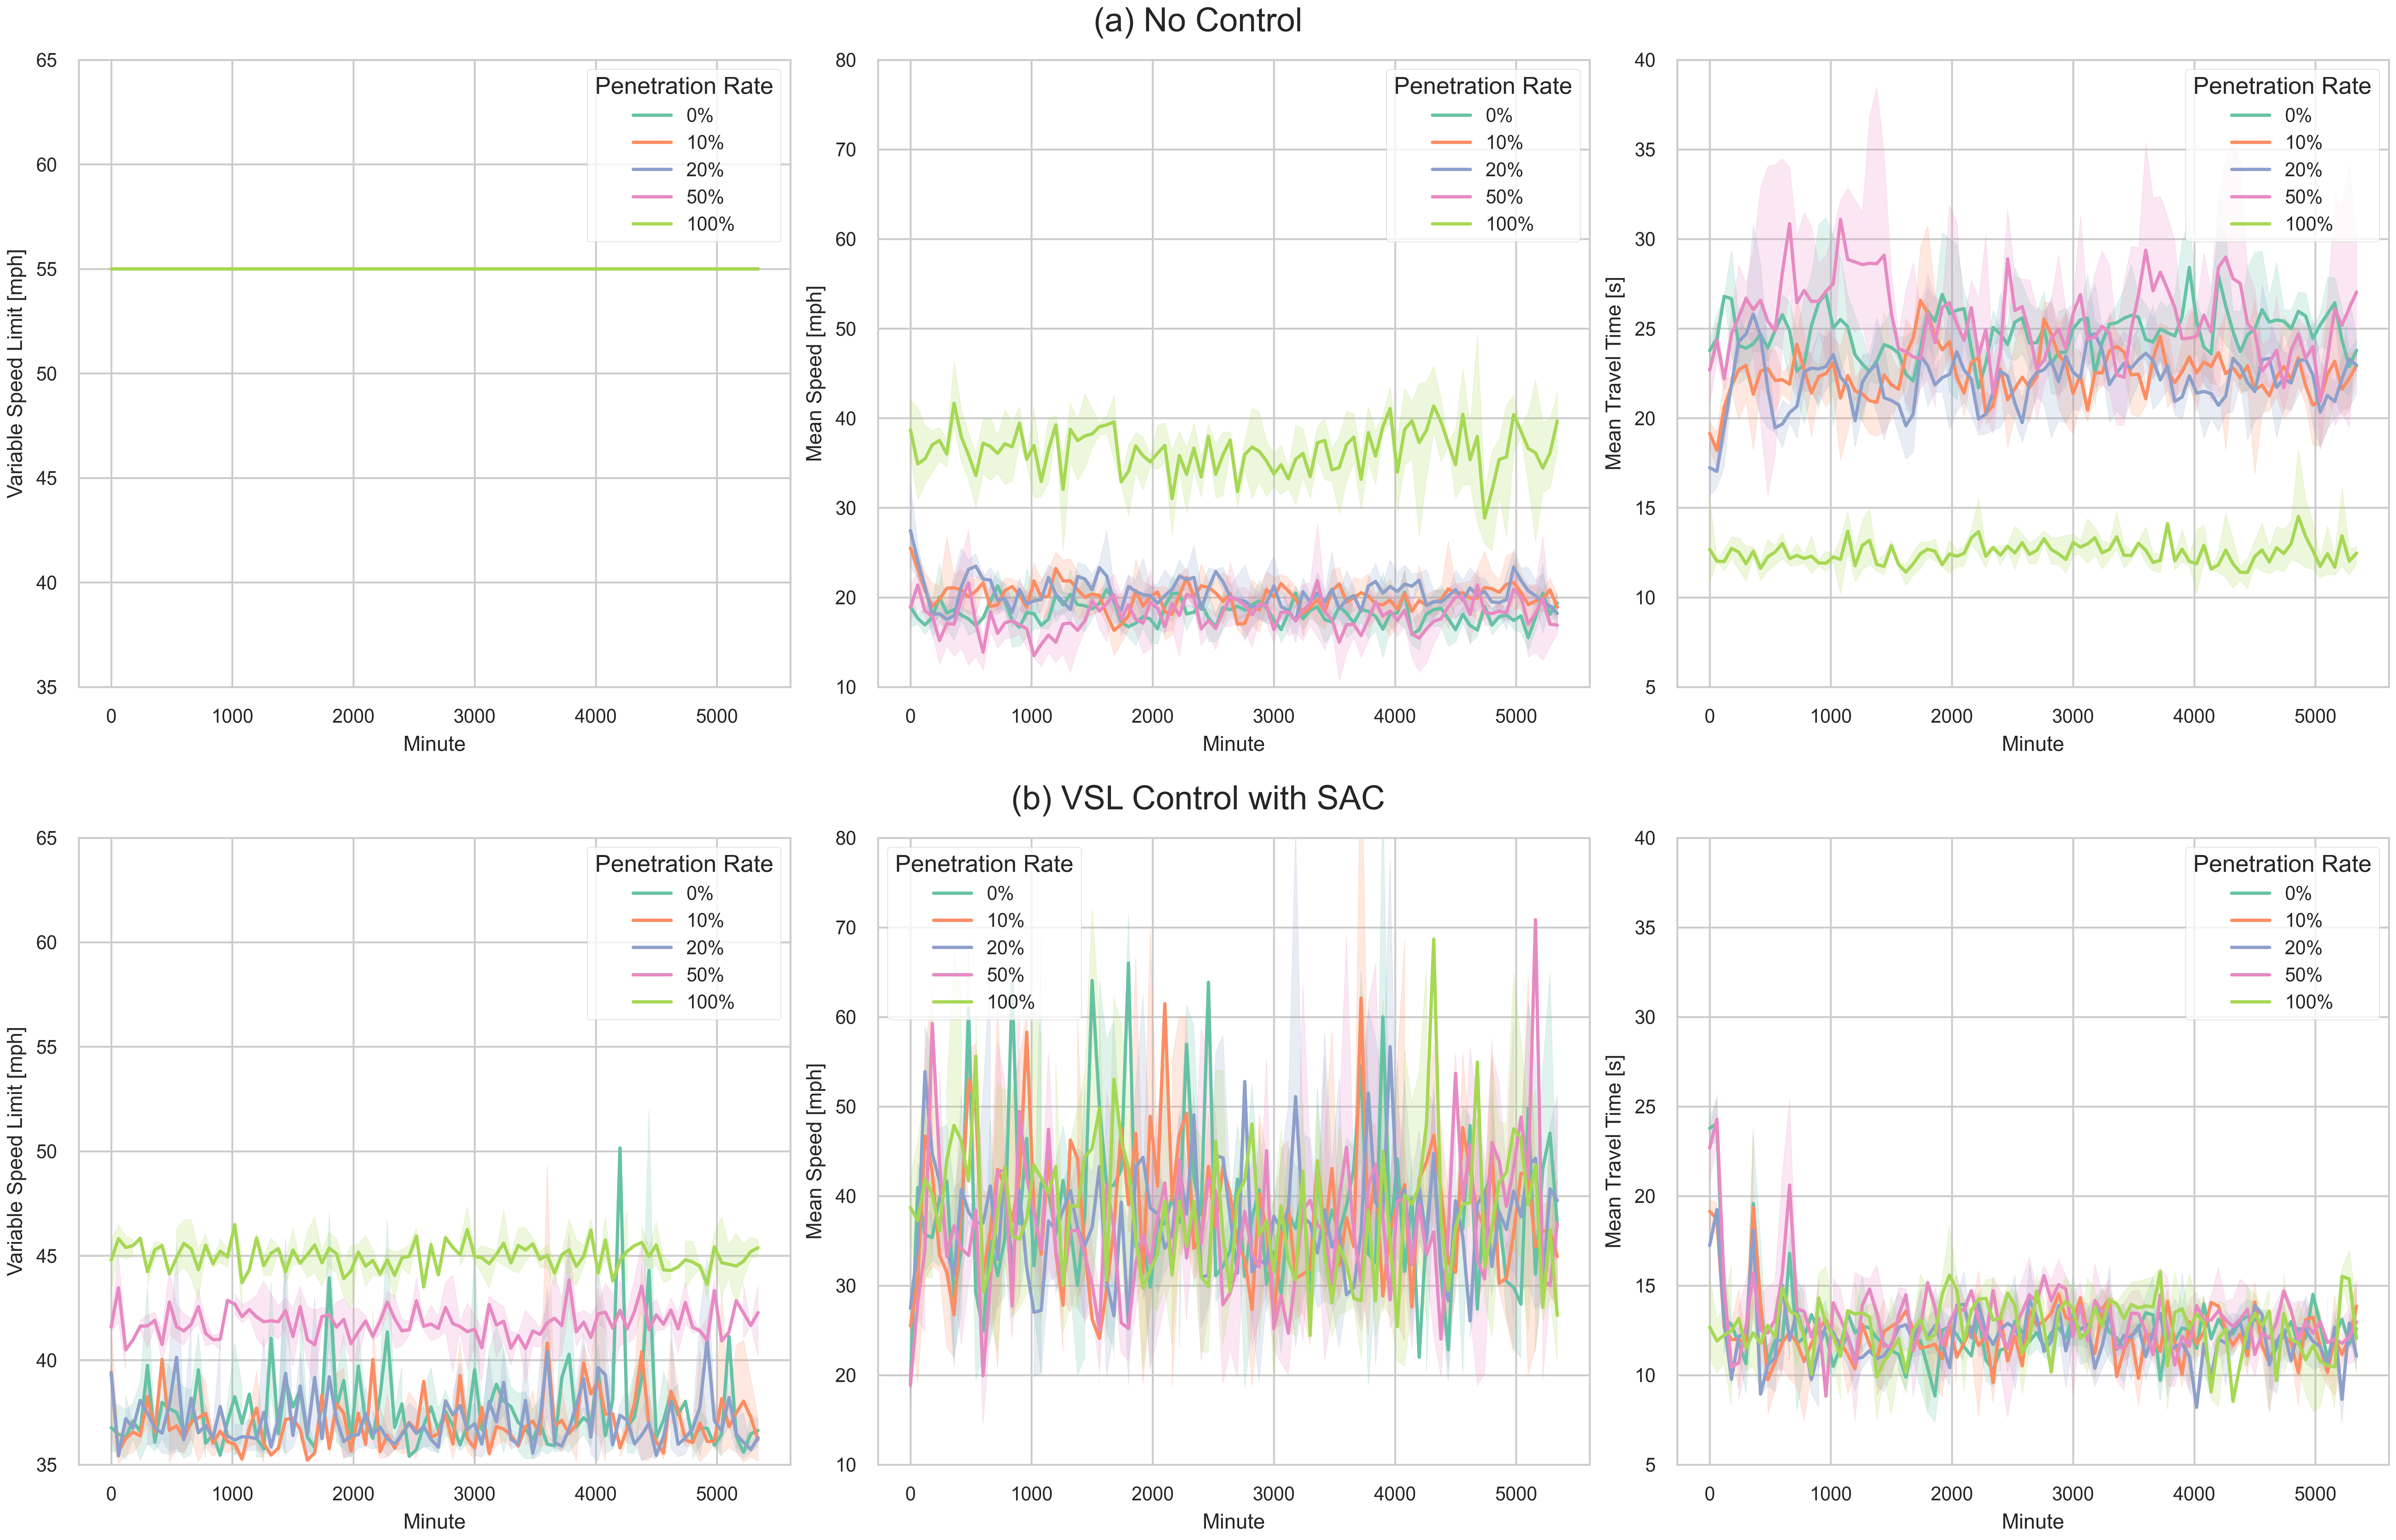
\includegraphics[width=\textwidth]{img/result.png}
    \caption{The variable speed limits for the upstream (left), average speed (middle), and average travel time (right) in the weaving area with (a) No VSL control and (b) SAC VSL Controller.}
    \label{fig:5}
\end{figure}

\section{Conclusions}

This paper proposes a VSL controller designed with the SAC reinforcement learning algorithm for mixed traffic flow environments,  where CAVs in the flow have better control and the ability to conform to the speed limit. The performance of the proposed method was examined using a microscopic simulation built with NGSIM trajectory data and the SUMO simulator. Parameters of the car-following and lane-changing models for HDVs are calibrated using the trajectory data to behave realistically in the SUMO microscopic simulator. CAV parameters are selected to satisfy the assumption of sound vehicle control and less deviation from the speed limit. The simulation results show that even without deploying CAVs, our proposed VSL controller can improve downstream traffic efficiency. However, increasing CAV deployment can make VSL obsolete at very high penetration rates. It is essential to investigate further the interaction between CAV deployment and VSL control in future work.

\bibliographystyle{unsrtnat}
\bibliography{references}  %%% Uncomment this line and comment out the ``thebibliography'' section below to use the external .bib file (using bibtex) .


%%% Uncomment this section and comment out the \bibliography{references} line above to use inline references.
% \begin{thebibliography}{1}

% 	\bibitem{kour2014real}
% 	George Kour and Raid Saabne.
% 	\newblock Real-time segmentation of on-line handwritten arabic script.
% 	\newblock In {\em Frontiers in Handwriting Recognition (ICFHR), 2014 14th
% 			International Conference on}, pages 417--422. IEEE, 2014.

% 	\bibitem{kour2014fast}
% 	George Kour and Raid Saabne.
% 	\newblock Fast classification of handwritten on-line arabic characters.
% 	\newblock In {\em Soft Computing and Pattern Recognition (SoCPaR), 2014 6th
% 			International Conference of}, pages 312--318. IEEE, 2014.

% 	\bibitem{hadash2018estimate}
% 	Guy Hadash, Einat Kermany, Boaz Carmeli, Ofer Lavi, George Kour, and Alon
% 	Jacovi.
% 	\newblock Estimate and replace: A novel approach to integrating deep neural
% 	networks with existing applications.
% 	\newblock {\em arXiv preprint arXiv:1804.09028}, 2018.

% \end{thebibliography}


\end{document}
